\documentclass[10pt,a4paper]{article}
\usepackage[utf8]{inputenc}
\usepackage{amsmath}
\usepackage{amsfonts}
\usepackage{amssymb}
\usepackage{wrapfig}
\usepackage{graphicx}
\usepackage{caption}
\usepackage{dirtytalk}
\usepackage[left=1.5cm,right=1.5cm,top=2cm,bottom=2cm]{geometry}


\usepackage{fancyhdr}
\pagestyle{fancy}


\renewcommand{\headrulewidth}{1pt}
%\fancyhead[C]{\textbf{page \thepage}}
%\fancyhead[L]{\leftmark}
%\fancyhead[R]{machin}

\fancyfoot[C]{\textbf{page \thepage}}
\fancyfoot[L]{\textsc{Thibaut VERCUEIL}}
\fancyfoot[R]{Internship Report}


\newcommand{\seas}{School of Engineering and Applied Sciences}
\newcommand{\hseas}{Harvard School of Engineering and Applied Sciences}
\renewcommand{\rmdefault}{phv} % Arial
\renewcommand{\sfdefault}{phv} % Arial

\title{{\Huge Internship ING4}\\ Report\\ \vspace{1cm} Harvard University}
\author{Thibaut Vercueil}


\begin{document}
\maketitle
\begin{abstract}
This is the abstract\end{abstract}
\newpage
\tableofcontents
\newpage
\section*{Acknowledgement}

\section{Introduction}
%----------------------------------
% PART I   ------------------------
%----------------------------------
\newpage
\part{Harvard University}


\section{History}

\subsection{Harvard University}
%TODO WHERE ??


\begin{wrapfigure}{R}{0.2\textwidth}
\centering

\includegraphics[width=0.15\textwidth]{harvardlogo.png}
\caption*{Havard seal}
\end{wrapfigure}
Harvard university is the most ancient university of the United States. It's located in Cambridge, Massachusetts, in Boston's suburb. It has been created in 1636 by vote of the Court of the Massachusetts Bay Colony. The school was name \textit{Harvard College} in 1639, in homage to John Harvard, who had left the school livre 779 and his library of some 400 books. John Harvard was the first donor to the school.\\
%MAYBE TALK ABOUT THE OTHER DONORS
During the following decades, Harvard University never ceased to grow up and it's now the richest University in the world with \$36.4 billion of endowment.

%TODO A graph with some figures

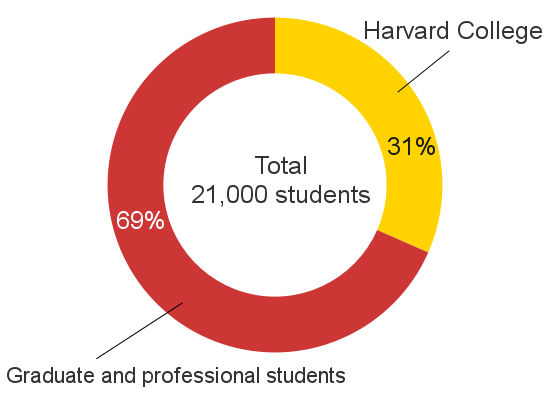
\includegraphics[width=0.3\textwidth]{images/fig1.png}

Harvard university include several universities, here is a list of the most important ones:\\
\begin{itemize}
  \item Faculty of Arts and Sciences composed by \\Harvard College \\Continuing Education \\Graduate School of Arts and Sciences \\Harvard John A. Paulson School of Engineering and Applied Sciences
\item Business School
\item Kennedy School of Government
\item Law School
\item Medical School
\item Radcliffe Institute
\item School of Education
\item Harvard T.H. Chan School of Public Health
\end{itemize}


\subsection{Harvard School of Engineering and Applied Sciences}
As you saw earlier ``beeing in Harvard'' without precising which university doesn't mean much, and so, during this in internship, I was affiliated to the Harvard School of Engineering and Applied Sciences, later called SEAS — Litte story: the school name changed during my journey, as Mr John A. Pauson did a donnation of \$ 400.000.000 to SEAS, so the school was rename after him.\\

The progenitor of the School of Engineering and Applied Sciences was called \textit{Lawrence Scientific School} and was founded in 1847. It was name for Abbott Lawrence, who donated \$50,000 (an unprecedented sum at the time) to create the institution. The was detached from Harvard College, which means it was independ financiery.
At this time, the School saw a diverse group of thinkers and professionals — astronomers, architects, naturalists, engineers, mathematicians, and even philosophers — pass through its doors.\\
At the end of the 19\textsuperscript{th} century, the school suffered the ``Competition'' from the new born Massachusset Institute of Technology (MIT) — Now one of the greatest engineering school in the world. The Harvard president of the time tried to merge the Harvard Scientific School with the MIT, vainly.\\
In 1901, despite the help of Gordon McKay, the school merged with Harvard College and lost his independance.\\

Later, the Harvard Lawrence Scientific School became \textit{The Division of Applied Science} and in 2007, it was rename as the \textit{Harvard School of Engineering and Applied Science}\\
It's a new start for the the School, Venkatesh Narayanamurti, Dean of Harvard School of Engineering and Applied Sciences at the time declared:\\
\say{\textit{Our transition from a Division to a School is not a departure from history—but in some sense, we are coming full circle. The Lawrence School, our progenitor, will be reborn in a new form appropriate for the 21st century.}}\\

Thus, strictly speaking, SEAS is a young school, only 8 years old, and in full growth. Thanks to the 4 milion dollars given by John Paulson, the school will expend and build laboratories in Allston, the city bordering Cambrigdge, on the other side of the river.\\

In order to realise the importance of Harvard engineering school in the world of sciences, here are a few examples of inventions made here:
\begin{itemize}
\item in 1919, the \textbf{crystal oscillator} came out of the Harvard Engineering School’s Cruft Laboratory, invented by George Washington Pierce
\item in 1938, the \textbf{largest cyclotron of the world} (at the time) was constructed at the Graduate School of Engineering's Gordon McKay Engineering Laboratory.
\item in 1977, Bill gates would have graduated from Harvard but he left the university  to found \textbf{Microsoft}, one of the biggest company in the world.
\item in 2004, \textbf{Facebook} was born in a dorm room of Harvard housing, created by Mark Zuckerberg, it's now the biggest social network ever created
\end{itemize}

\subsection{Mazur group}

\hseas{} is composed by several reseach groups. This summer, I worked with the group of professor Eric Mazur, Balkanski Professor of Physics and Applied Physics and Area Dean for Applied Physics.\\
Professor Mazur founded the group in 1111%I DON'T KNOW
to study the dynamics of molecules, chemical reactions, and condensed matter on very short timescales — down to femtoseconds ($10^{-15}$ second). Physics in this ultrafast regime is studied using light, specifically very short laser pulses. So the mazur group works with femtoseconds lasers.\\
In addition to the work in optical physics, The Mazur Group is very active in research about education. In 1990, Eric Mazur began developing Peer Instruction, a method for teaching large lecture classes interactively. He is the author of \textit{Peer Instruction: A User's Manual} (Prentice Hall, 1997), a book that explains how to teach large lecture classes interactively.

\newpage
\section{Organization}
\subsection{Main organization of the university}
Harvard University is huge. It's composed by a dozen of universities and it's under the direction of the president Drew Gilpin Faust and the provost Alan M. Garber.\\

Harvard is known to be a decentralized organization. Each constituent faculties has a lot of independence. This mean each faculties set their own academic standards and manage their own budgets. Each facultie is directed by the faculty dean whose role is to manage the matters of the facutly\\

Here you can see a chart representing the several faculties composing Harvard University (The one in which I worked is highlighted):\\
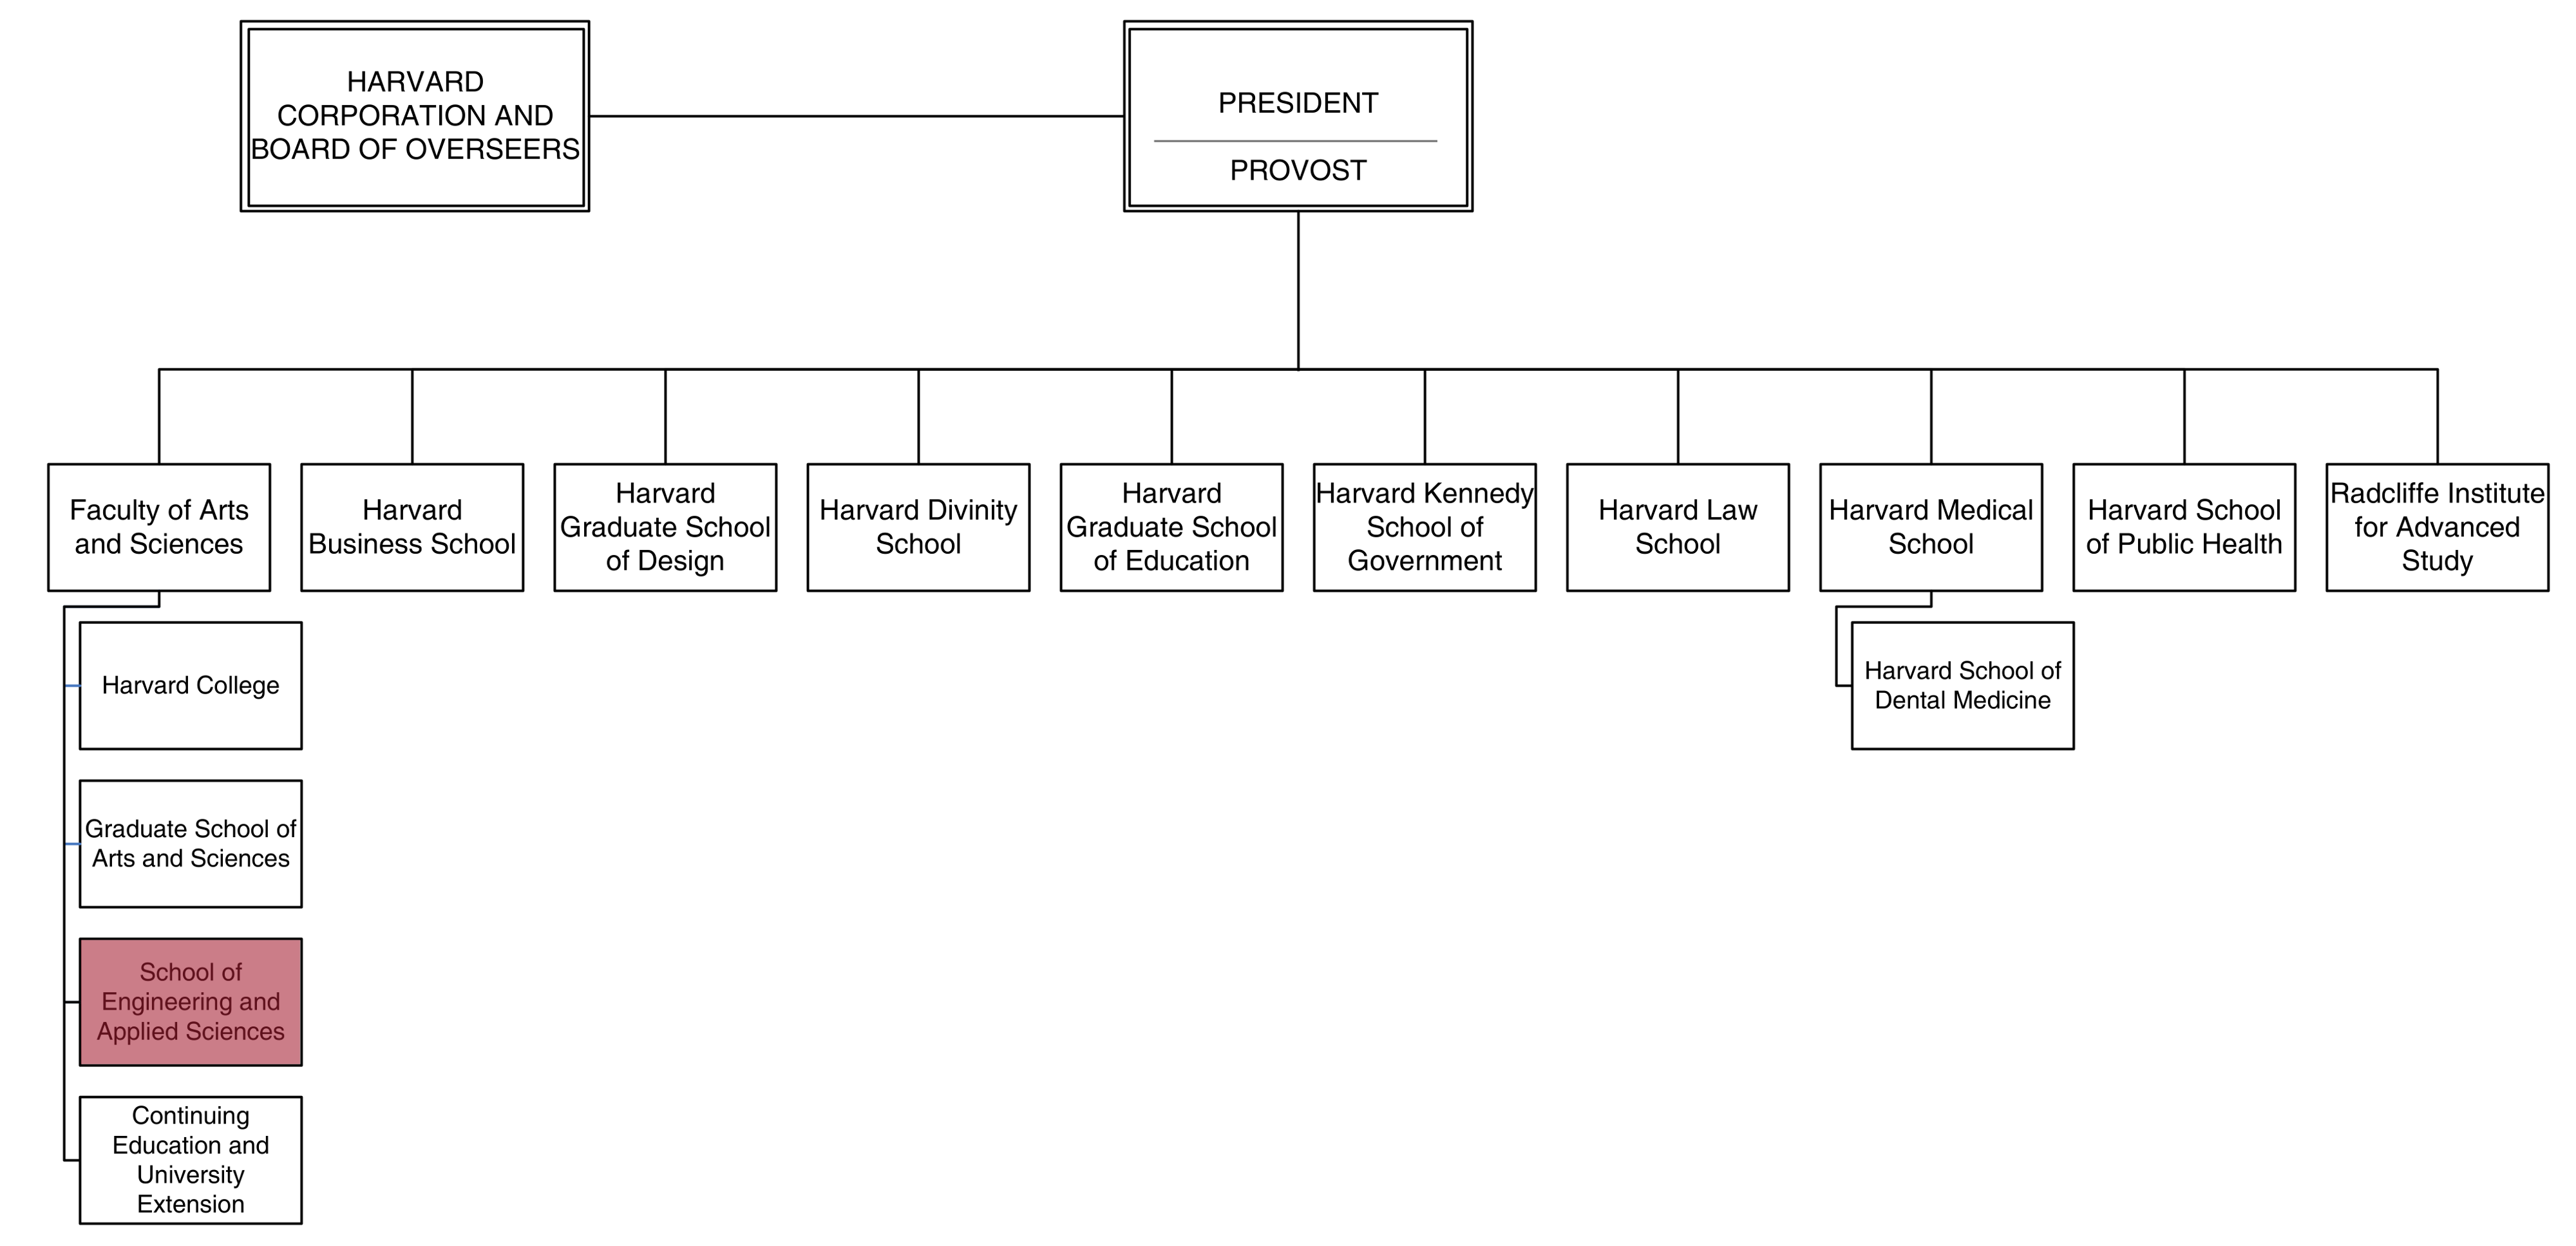
\includegraphics[width=1\textwidth]{images/chart1.png}

%Comment le président d'Harvard est il nommé ?
However, despite this decentralized management, the roles of the president and the provost are really important.\\

\textbf{The president} of Harvard university has two hats: Chief administrator of the university and the \textit{ex officio} chairman of the Harvard Corporation.
The president plays an important part in university-wide planning and strategy. She names a faculty's dean the university's provost, and she grants tenure to recommended professors. However, she is expected to make such decisions after extensive consultation with faculty members.\\
Moreover, as the leader of one of the most prominent universities in the world, Harvard presidents have influenced educational practices nationwide.\\

\textbf{The provost} of Harvard serves as chief academic officer. He works with the President to oversee academic policies and activities university-wide. The Office of the Provost works closely with the University’s academic and administrative leaders to: foster interfaculty collaboration, improve Harvard’s performance in building a diverse pipeline of scholars and in developing scholars at all stages of the academic career ladder, advance university-wide approaches to compliance and research policy, support University cultural and artistic entities and projects; oversee and coordinate the University’s international activities; support faculty, students, and academic professionals in advancing innovations in teaching and learning; and oversee activities pertaining to intellectual property, technology transfer, research collaborations with industry, and trademark licensing\footnote{provost.harvard.edu}.\\
%AS YOU CAN SEE _ON_ THIS CHART
The chart bellow represent the organization of the Harvard's central administration:\\
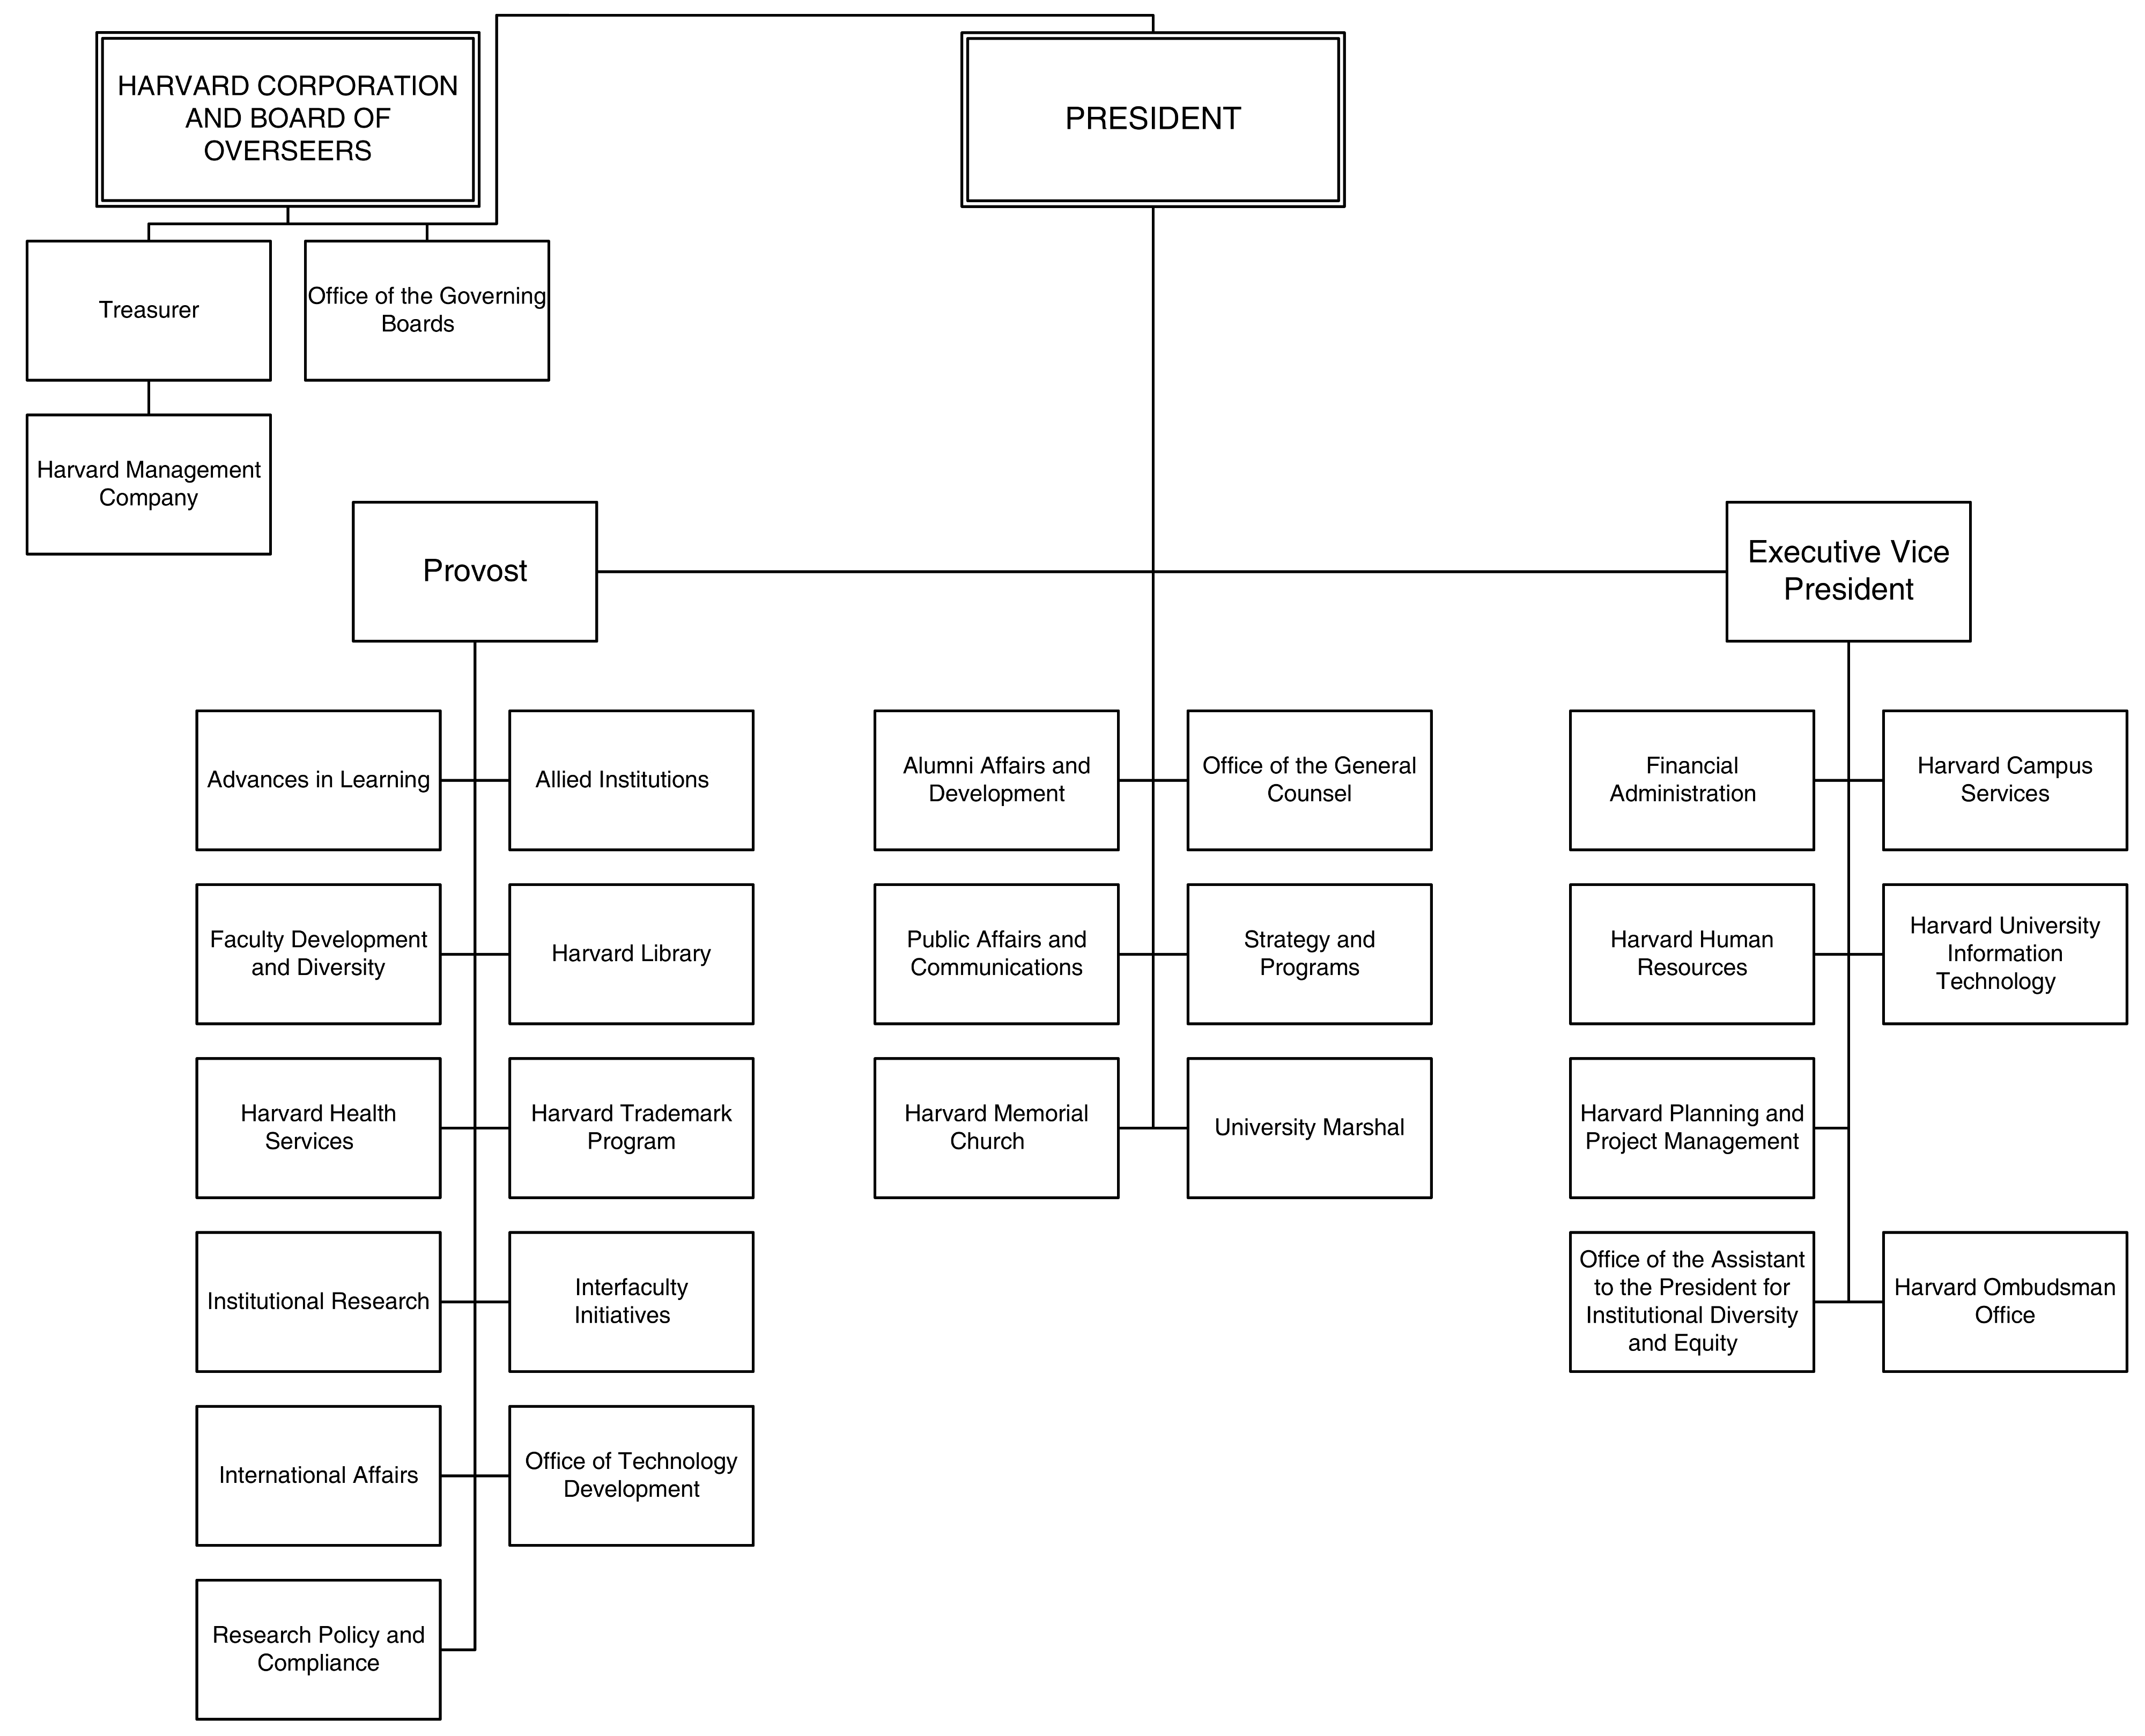
\includegraphics[width=1\textwidth]{images/chart2.png}
%TODO: COMMENT THIS CHART !










\end{document}
